\section{Linear Regression}\label{sec:linreg}
Suppose you have a data set $\mathcal{L}$ consisting of the data
$\mathbf{X}_\mathcal{L}=\{(y_i, x_i), i=0\ldots n-1\}$. Each point is associated
with a scalar target $y_i$, and a vector $\bs{x}$ containing values for $p$ input
features. Assuming the target variable $y_i$ is linear in the inputs, it can be
written as a linear function of the features, given by
\begin{equation}\label{eq:ols-target}
y_i = w_0 x_{i,0} + w_1 x_{i,1} + ... + w_{p-1} x_{i, p-1} + \epsilon_i,
\end{equation}
where $\bs{w} = (w_0, w_1, \dots, w_{p-1})^T$ is a vector of length
$p$ containing unknown values, and $\epsilon$ are the errors in our estimate.
This gives us a system of linear equations, which can be written in matrix form as
\begin{equation}\label{eq:ols-target-mat}
  \bs{y} = \bs{Xw} + \bs{}{\epsilon},
\end{equation}
where
\begin{equation}
\vec{X} = \left[
\begin{matrix}
x_{0,0} & x_{0,1} & x_{0,2} & ... & x_{0,p-1}\\
x_{1,0} & x_{1,1} & x_{1,2} & ... & x_{1,p-1}\\
x_{2,0} & x_{2,1} & x_{2,2} & ... & x_{2,p-1}\\
\vdots & \vdots & \vdots & \ddots & \vdots\\
x_{n-1,0} & x_{n-1,1} & x_{n-1,2} & ... & x_{n-1,p-1}
\end{matrix}
\right]
\end{equation}
The unknown values $\bs{w}$ are commonly referred to as \textit{weights} in machine 
learning literature. To find the best possible weights $\bs{w}$ we want a suitable
quantity to optimize - a \textbf{cost function}, $\mathcal{C}$ (also referred to as an
\textbf{objective function}). An example of such a function is the squared error - or the Euclidian vector norm, defined as
\begin{equation}
	L_2(\bs{x}) =||\bs{x}||_2 = \left(\sum x_i^2\right)^{\frac{1}{2}}.
\end{equation}
From this we define the cost function
\begin{equation}
	\mathcal{C} = || \bs{\hat{y}} - \bs{y} ||_2 ^2.
\end{equation}
In machine learning, it is most common to cast the optimization as a minimization problem
("minimize the cost"). Our task is then to find an approximation
\begin{equation}\label{eq:ols-approximation}
	\bs{\hat{y}} = \bs{Xw}
\end{equation}
which minimizes this cost function.
To find the minimum we need a differentiation. To simplify that process, we rewrite the cost function on matrix form
\begin{align*}
\mathcal{C} &= || \bs{\hat{y}} - \bs{y} ||_2 ^2, \\
\mathcal{C} &= ( \bs{\hat{y}} - \bs{Xw})^T( \bs{\hat{y}} - \bs{Xw}).
\end{align*}
To minimize we take the derivative with respect to the weights $\bs{w}$,
and find the minima by setting the derivative equal to zero
\begin{align}
\nabla _{\bs{w}}\mathcal{C} &= \nabla _{\bs{w}} ( \bs{\hat{y}} - \bs{Xw})^T( \bs{\hat{y}} - \bs{Xw}), \\
&= -2\bs{X}^T\bs{\hat{y}} + 2\bs{X}^T\bs{X}\bs{w}, \\
\bs{0} &= -2\bs{X}^T\bs{\hat{y}} + 2\bs{X}^T\bs{X}\bs{w}, \\
\bs{X}^T\bs{\hat{y}} &= \bs{X}^T\bs{X}\bs{w}, \\
\bs{w} &=(\bs{X}^T\bs{X})^{-1} \bs{X}^T\bs{\hat{y}}. \label{eq:ols}
\end{align}
This requires matrix \(\vec{X}^T\vec{X}\) to be invertible to get the solution 
\cite{James2000}.

The residuals $\bs{\epsilon}$ are given by
$$\bs{\epsilon} = \bs{y}-\bs{\hat{y}} = \bs{y}-\bs{X}\bs{w},$$
and with 
$$\bs{X}^T\left( \bs{y}-\bs{X}\bs{w}\right)= 0,$$
we have
$$\bs{X}^T\bs{\epsilon}=\bs{X}^T\left( \bs{y}-\bs{X}\bs{w}\right)= 0,$$
meaning that the solution for $\bs{w}$ is the one which minimizes the residuals.
This method of regression is known as Ordinary Least Squares.

\section{Over- and underfitting}\label{sec:overfitting}
In machine learning, when fitting a model to a data set the goal is nearly always to predict 
values or classify samples from regions of data the model has not seen. This is not a simple task,
especially taking into consideration that data is rarely, if ever, noiseless. When extrapolating to 
unseen regions we must take steps to ensure the model complexity is appropriate - we want it to fit 
the signal, not the noise. First off - what do the terms "overfit" and "underfit" mean?
An overfit model will typically perform well during the fitting procedure, but when presented with
data outside the fitted region its performance decreases considerably.
An underfit model lacks the expressive power to capture core signal variations in the data.
Mehta et. al \cite{Mehta2019} demonstrates this concept through polynomial regression.

In machine learning literature and practice, you will encounter the concept of
splitting the available data into two - training data and test data. We fit, or 'train'
the model on the training data, and then assess the performance of the model on the 
test data. This practice lets us evaluate whether the model is overfitting to unseen
data by comparing performance on the training data and test data.

\section{The Bias-Variance Tradeoff}\label{sec:bias-variance}
Considering the same dataset $\mathcal{L}$ consisting of the data,
let us assume that the true data is generated from a noisy model

$$\mathbf{y}=f(\bs{x}) + \bs{\epsilon},$$
where $\epsilon$ is normally distributed with mean zero and standard deviation $\sigma^2$.

In our derivation of the ordinary least squares method we defined
an approximation (\ref{eq:ols-approximation}) to the function $f$ in terms of the 
weights $\bs{w}$ and the input matrix $\bs{X}$ which together define our model,
that is $\bs{\hat{y}}=\bs{X}\bs{w}$. 

Thereafter we found the parameters $\bs{w}$ by optimizing the means squared error via the so-called cost function

$$\mathcal{C}(\bs{X},\bs{w}) =\frac{1}{n}\sum_{i=0}^{n-1}(y_i-\hat{y}_i)^2=\mathbb{E}\left[(\bs{y}-\bs{\hat{y}})^2\right].$$

We can rewrite this as 
$$\mathbb{E}\left[(\bs{y}-\bs{\hat{y}})^2\right]=\frac{1}{n}\sum_i(f_i-\mathbb{E}\left[\bs{\hat{y}}\right])^2+\frac{1}{n}\sum_i(\hat{y}_i-\mathbb{E}\left[\bs{\hat{y}}\right])^2+\sigma^2.$$

The three terms represent the square of the bias of the learning
method, which can be thought of as the error caused by the simplifying
assumptions built into the method. The second term represents the
variance of the chosen model and finally the last terms is variance of
the error $\bs{\epsilon}$.

For a derivation of this equation, we refer to the work of Mehta et. al \cite{Mehta2019}.
The authors also provide a list of universal lessons to keep in mind, which we quote here:

\begin{itemize}
	\item Fitting is not predicting. Fitting existing data well is fundamentally
	different from making predictions about new data.
	\item Using a complex model can result in overfitting. Increasing a model's
	complexity  (i.e number of fitting parameters) will usually yield better results
	on the training data. However when the training data size is small and the data
	are noisy, this results in \textit{overfitting} and can substantially degrade the
	predictive performance of the model.
	\item For complex datasets and small training sets, simple models can be better
	at prediction complex models due to the bias-variance tradeoff. It takes less
	data to train a simple model than a complex one. Therefore, even though the 
	correct model is guaranteed to have better predictive performance for an infinite
	amount of training data (less bias), the training errors stemming from finite-size
	sampling (variance) can cause simpler models to outperform the more complex model
	when sampling is limited.

\end{itemize}

% Derivation from lecture notes here.
%to recall that the variance of $\bs{y}$ and $\bs{\epsilon}$ are both equal to $\sigma^2$. 
%The mean value of $\bs{\epsilon}$ is by definition equal to zero. Furthermore, the function $f$ is not a stochastics variable, idem for $\bs{\hat{y}}$.
%We use a more compact notation in terms of the expectation value
%$$\mathbb{E}\left[(\bs{y}-\bs{\hat{y}})^2\right]=\mathbb{E}\left[(\bs{f}+\bs{\epsilon}-\bs{\hat{y}})^2\right],$$
%and adding and subtracting $\mathbb{E}\left[\bs{\hat{y}}\right]$ we get
%$$\mathbb{E}\left[(\bs{y}-\bs{\hat{y}})^2\right]=\mathbb{E}\left[(\bs{f}+\bs{\epsilon}-\bs{\hat{y}}+\mathbb{E}\left[\bs{\hat{y}}\right]-\mathbb{E}\left[\bs{\hat{y}}\right])^2\right],$$
%which, using the abovementioned expectation values can be rewritten as
%$$\mathbb{E}\left[(\bs{y}-\bs{\hat{y}})^2\right]=\mathbb{E}\left[(\bs{y}-\mathbb{E}\left[\bs{\hat{y}}\right])^2\right]+\mathrm{Var}\left[\bs{\hat{y}}\right]+\sigma^2,$$
%that is the rewriting in terms of the so-called bias, 
%the variance of the model $\bs{\hat{y}}$ and the variance of $\bs{\epsilon}$.

\section{Regularization}\label{section:regularization}
With the computing resources available today, increasing model complexity to deal 
with underfitting is usually a simple task. However, this computational freedom 
has led to overfitting being the common challenge to overcome.

\section{Logistic Regression}\label{seq:logistic}
Differently to linear regression, classification problems
are concerned with outcomes taking the form of discrete variables.
For a specific physical problem, we'd like to identify its state, say whether
it is an ordered of disordered system. (cite?) One of the most basic examples
of a classifier algorithm is logistic regression.

For a logistic regressor to improve it needs a way to
track its performance. This is the purpose of a cost function. Essentially,
the cost function says something about how wrong the model is in classifying the
input. The objective in machine learning, and logistic regression, is then to minimize
this error.

The cost function used in this project is called the \textbf{cross-entropy}, or the
'negative log likelihood', and takes the form
\begin{equation}\label{eq:cross-entropy}
	\mathcal{C}(\bs{w})=-\sum_{i=1}^n  \left(y_i(w_0+w_1x_i) -\log{(1+\exp{(w_0+w_1x_i)})}\right)
\end{equation}

\section{Gradient Descent}\label{seq:gradient}
Minimizing the cost function is done using Gradient Descent.
The gist of it is that to optimize the weights or coefficients,
and biases to minimize the cost function, we can change their values to

\begin{equation}\label{eq:delta-c}
	\frac{\partial \mathcal{C}(\bs{w})}{\partial \bs{w}} = -\bs{X}^T\left(\hat{y}-\hat{p}\right)
\end{equation}

\subsection{Stochastic Gradient Descent}
The stochastic gradient descent method address some of the shortcomings
of the normal gradient descent method. The gradient descent method is
for instance sensitive to the choice of learning rate (cite?).

The underlying idea of stochastic gradient descent comes from observing
that the cost function we want to minimize, almost always can be written as
a sum over \(n\) data points. (cite?). Which gives

\begin{equation}
	C(w) = \sum\limits_{i=1}^n c_i (\mathbf{x}_iw)
\end{equation} (cite?)

This means that we also can find the gradient as a sum over i gradients
as follows:

\begin{equation}
	\Delta_{w} C(w) = \sum\limits_{i}^n \Delta_{w}c_i (\mathbf{x}_iw)
\end{equation} (cite?)

Randomness is included by only taking the gradient on a subset of data.

\section{Neural Networks}
Artificial neural networks (ANN) are computational systems that can learn to
perform tasks by considering examples, generally without being
programmed with any task-specific rules. It is supposed to mimic a
biological system, wherein neurons interact by sending signals in the
form of mathematical functions between layers. All layers can contain
an arbitrary number of neurons, and each connection is represented by
a weight variable.
The field of artificial neural networks has a long history of
development, and is closely connected with the advancement of computer
science and computers in general.

In natural sciences, ANNs have already found numerous applications.
In statistical physics, they have been applied to detect
phase transitions in 2D Ising and Potts models, lattice gauge
theories, and different phases of polymers, or solving the
Navier-Stokes equation in weather forecasting.  Deep learning has also
found interesting applications in quantum and nuclear physics.

The applications are not limited to the natural sciences. There is a
plethora of applications in essentially all disciplines, from the
humanities to life science and medicine.

\subsection{Artificial Neurons}
A model of artificial neurons was first developed by McCulloch and Pitts in 1943 
\cite{McCulloch1943} to study signal
processing in the brain and has later been refined by others. The
general idea is to mimic neural networks in the human brain, which is
composed of billions of neurons that communicate with each other by
sending electrical signals.  Each neuron accumulates its incoming
signals, which must exceed an activation threshold to yield an
output. If the threshold is not overcome, the neuron remains inactive,
i.e. has zero output. This behaviour inspired a simple mathematical model for an artificial neuron.

\begin{equation}\label{eq:artificial-neuron}
 y = f\left(\sum_{i=1}^n w_ix_i\right) = f(z)
\end{equation}

Here, the output $y$ of the neuron is the value of its activation function,
which receives as input a weighted sum of signals $x_i, \dots ,x_n$ received by $n$ other neurons.
Neurons are often referred to as "nodes" or "units" in machine learning literature,
and we will use these interchangeably in the following sections.

\subsection{The neural network}
A network of only one neuron such as the one described above is typically referred
to as a \textit{perceptron}. The simplest network structure contains a
single layer of N such nodes, and is most often called a \textit{single-layer perceptron}.
Adding additional layers of nodes, so-called \textit{hidden layers}, results in a
type of feed-forward neural network (FFNN), typically referred to as a Multilayer Perceptron (MLP)
(see figure \ref{fig:theory-mlp}). The example is also a fully connected network, as every
node in a layer is connected to every node in the next. The name "feed-forward" stems from
the fact that information flows in only one direction: forward through the layers.
\def\layersep{2.5cm}
% https://texample.net/tikz/examples/neural-network/
\begin{figure}
    \centering
    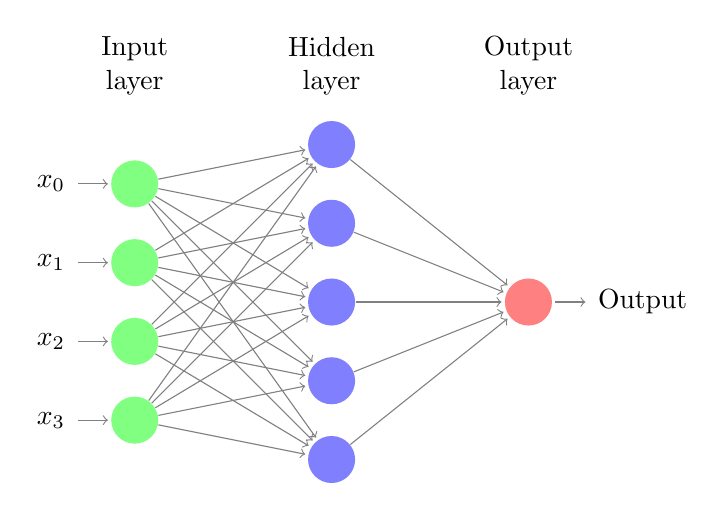
\begin{tikzpicture}[shorten >=1pt,->,draw=black!50, node distance=\layersep]
        \tikzstyle{every pin edge}=[<-,shorten <=1pt]
        \tikzstyle{neuron}=[circle,fill=black!25,minimum size=17pt,inner sep=0pt]
        \tikzstyle{input neuron}=[neuron, fill=green!50];
        \tikzstyle{output neuron}=[neuron, fill=red!50];
        \tikzstyle{hidden neuron}=[neuron, fill=blue!50];
        \tikzstyle{annot} = [text width=4em, text centered]
        
        % Draw the input layer nodes
        \foreach \name / \y in {0,...,3}
        % This is the same as writing \foreach \name / \y in {1/1,2/2,3/3,4/4}
        \node[input neuron, pin=left: $x_{\y}$] (I-\name) at (0,-\y) {};
        
        % Draw the hidden layer nodes
        \foreach \name / \y in {0,...,4}
        \path[yshift=0.5cm]
        node[hidden neuron] (H-\name) at (\layersep,-\y cm) {};
        
        % Draw the output layer node
        \node[output neuron,pin={[pin edge={->}]right:Output}, right of=H-2] (O) {};
        
        % Connect every node in the input layer with every node in the
        % hidden layer.
        \foreach \source in {0,...,3}
        \foreach \dest in {0,...,4}
        \path (I-\source) edge (H-\dest);
        
        % Connect every node in the hidden layer with the output layer
        \foreach \source in {0,...,4}
        \path (H-\source) edge (O);
        
        % Annotate the layers
        \node[annot,above of=H-0, node distance=1cm] (hl) {Hidden layer};
        \node[annot,left of=hl] {Input layer};
        \node[annot,right of=hl] {Output layer};
    \end{tikzpicture}
    \caption{\label{fig:theory-mlp}An example of a simple, feed-forward neural network architecture. Each input
    $x_i$ is fed to each node in the hidden layer, where the value of the activation
    function $f(z)$ is calculated and passed on to the output layer. In this case the
    output layer consists of only one node.
    }
\end{figure}
First, for each node $i$ in the first hidden layer, we calculate a weighted sum $z_i^1$ of the input coordinates $x_j$,

\begin{equation} 
	z_i^1 = \sum_{j=1}^{M} w_{ij}^1 x_j + b_i^1
\end{equation}
Here $b_i$ is the \textit{bias} which is needed in
case of zero activation weights or inputs. How to fix the biases and
the weights will be discussed below.  The value of $z_i^1$ is the
argument to the activation function $f_i$ of each node $i$, The
variable $M$ stands for all possible inputs to a given node $i$ in the
first layer.  We define  the output $y_i^1$ of all neurons in layer 1 as

\begin{equation}\label{eq:output-layer}
	y_i^1 = f(z_i^1) = f\left(\sum_{j=1}^M w_{ij}^1 x_j  + b_i^1\right)
\end{equation}
where we assume that all nodes in the same layer have identical
activation functions, hence the notation $f$. In general, we could assume in the more general case that different layers have different activation functions.
In this case we would identify these functions with a superscript $l$ for the $l$-th layer,

\begin{equation}\label{eq:general-layer}
	y_i^l = f^l(u_i^l) = f^l\left(\sum_{j=1}^{N_{l-1}} w_{ij}^l y_j^{l-1} + b_i^l\right)
\end{equation}
where $N_l$ is the number of nodes in layer $l$. When the output of
all the nodes in the first hidden layer are computed, the values of
the subsequent layer can be calculated and so forth until the output
is obtained.

The output of neuron $i$ in layer 2 is thus,

\begin{align}\label{eq:output-layer-2}
	y_i^2 &= f^2\left(\sum_{j=1}^N w_{ij}^2 y_j^1 + b_i^2\right) \\
	&= f^2\left[\sum_{j=1}^N w_{ij}^2f^1\left(\sum_{k=1}^M w_{jk}^1 x_k + b_j^1\right) + b_i^2\right]
\end{align}
where we have substituted $y_k^1$ with the inputs $x_k$. Finally, the ANN output reads

\begin{align}
	y_i^3 &= f^3\left(\sum_{j=1}^N w_{ij}^3 y_j^2 + b_i^3\right) \\
	&= f_3\left[\sum_{j} w_{ij}^3 f^2\left(\sum_{k} w_{jk}^2 f^1\left(\sum_{m} w_{km}^1 x_m + b_k^1\right) + b_j^2\right)
	+ b_1^3\right]
\end{align}

We can generalize this expression to an MLP with $l$ hidden
layers. The complete functional form is,

\begin{align}\label{eq:complete-nn}
&y^{l+1}_i = f^{l+1}\left[\!\sum_{j=1}^{N_l} w_{ij}^3 f^l\left(\sum_{k=1}^{N_{l-1}}w_{jk}^{l-1}\left(\dots f^1\left(\sum_{n=1}^{N_0} w_{mn}^1 x_n+ b_m^1\right)\dots\right)+b_k^2\right)+b_1^3\right] &&
\end{align}

which illustrates a basic property of MLPs: The only independent
variables are the input values $x_n$.
This confirms that an MLP, despite its quite convoluted
mathematical form, is nothing more than an analytic function, specifically a
mapping of real-valued vectors $\bs{x} \in \mathbb{R}^n \rightarrow
\bs{y} \in \mathbb{R}^m$.

Furthermore, the flexibility and universality of an MLP can be
illustrated by realizing that the expression is essentially a nested
sum of scaled activation functions of the form
\begin{equation}
 f(x) = c_1 f(c_2 x + c_3) + c_4
\end{equation}

where the parameters $c_i$ are weights and biases. By adjusting these
parameters, the activation functions can be shifted up and down or
left and right, change slope or be rescaled which is the key to the
flexibility of a neural network.

We will now introduce a more convenient notation for the activations in an ANN. 
We can represent the biases and activations
as layer-wise column vectors $\bs{b}_l$ and $\bs{y}_l$, so that the $i$-th element of each vector 
is the bias $b_i^l$ and activation $y_i^l$ of node $i$ in layer $l$ respectively. 

We have that $\bs{W}_l$ is an $N_{l-1} \times N_l$ matrix, 
while $\bs{b}_l$ and $\bs{y}_l$ are $N_l \times 1$ column vectors. 
With this notation, the sum becomes a matrix-vector multiplication, and we can write
the equation for the activations of hidden layer 2 (assuming three nodes for simplicity) as
\begin{equation}
 \bs{y}_2 = f_2(\bs{W}_2 \bs{y}_{1} + \bs{b}_{2}) = 
 f_2\left(\left[\begin{array}{ccc}
    w^2_{11} &w^2_{12} &w^2_{13} \\
    w^2_{21} &w^2_{22} &w^2_{23} \\
    w^2_{31} &w^2_{32} &w^2_{33} \\
    \end{array} \right] \cdot
    \left[\begin{array}{c}
           y^1_1 \\
           y^1_2 \\
           y^1_3 \\
          \end{array}\right] + 
    \left[\begin{array}{c}
           b^2_1 \\
           b^2_2 \\
           b^2_3 \\
          \end{array}\right]\right).
\end{equation}

The activation of node $i$ in layer 2 is
\begin{equation}
 y^2_i = f_2\Bigr(w^2_{i1}y^1_1 + w^2_{i2}y^1_2 + w^2_{i3}y^1_3 + b^2_i\Bigr) = 
 f_2\left(\sum_{j=1}^3 w^2_{ij} y_j^1 + b^2_i\right).
\end{equation}

This is not just a convenient and compact notation, but also a useful
and intuitive way to think about MLPs: The output is calculated by a
series of matrix-vector multiplications and vector additions that are
used as input to the activation functions. For each operation
$\bs{W}_l \bs{y}_{l-1}$ we move forward one layer.

\subsection{Types of neural networks}

\subsubsection*{Convolutional Neural Network}

A different variant of FFNNs are \textit{convolutional neural networks}
(CNNs), which have a connectivity pattern inspired by the animal
visual cortex. Individual neurons in the visual cortex only respond to
stimuli from small sub-regions of the visual field, called a receptive
field. This makes the neurons well-suited to exploit the strong
spatially local correlation present in natural images. The response of
each neuron can be approximated mathematically as a convolution
operation.  (figure to come)

Convolutional neural networks emulate the behaviour of neurons in the
visual cortex by enforcing a *local* connectivity pattern between
nodes of adjacent layers: Each node in a convolutional layer is
connected only to a subset of the nodes in the previous layer, in
contrast to the fully-connected FFNN.  Often, CNNs consist of several
convolutional layers that learn local features of the input, with a
fully-connected layer at the end, which gathers all the local data and
produces the outputs. They have wide applications in image and video
recognition.


\subsection{Backpropagation}

\section{Assessing the Performance of Models}
If classification accuracy is not enough to gauge whether a model is
performing well, or well in the desired way, alternative way to measure
performance must be explored. For cases of imbalanced data there are a few
widely used methods that reveal information about the model that the simple
accuracy metric can't.

\subsection{Imbalanced Data in Classification}
The physical world is rarely balanced.

A common challenge in classification is imbalanced data, in which a large
amount of the labeled data belongs to just one or a few of the classes.
For binary classification, if 90\% of the data belongs to one of the classes,
then the classifier is likely to end up placing every single
input in that class, as it will bring its accuracy to 90\%. Technically, this
accuracy is correct, but it's not very useful since the decision isn't at all
affected by the features of the input. Accuracy alone isn't a good enough
measure of performance to reveal this.

\subsection{Confusion Matrix}
A confusion matrix is an n by n matrix containing correct classifications
on the diagonal, and false positives and negatives in the off-diagonal elements.
An example of such a matrix could be the following table:
\begin{table}[h]
    \centering
    \begin{tabular}{c|c|c|c}
     & True Cat & True Dog & True Rabbit \\
    \hline
    Predicted Cat & \textbf{5} & 2 & 0 \\
    \hline
    Predicted Dog & 3 & \textbf{3} & 2 \\
    \hline
    Predicted Rabbit & 0 & 1 & \textbf{11} \\
\end{tabular}
\caption{Confusion matrix for an example classification where the classes
         are Cat, Dog and Rabbit. Correct classifications in bold.}
\label{tab:confmat-example}
\end{table}
In the table above (\ref{tab:confmat-example}), the diagonal elements
$i = j$ are the correct classifications, while the other elements correspond
to cases where the model predicted class $i$ but should've predicted class $j$.
The confusion matrix thus gives information about false positives and false
negatives, in addition to classification accuracy. This is very useful
in cases where for example false positives can be readily ignored or filtere
later, but false negatives may have severe consequences. An example of this
could be detection of cancer, in which a false positive can be ruled out
from further testing, while a false negative may lead to a patient being sent
home when actually needing help. For a more in-depth look at confusion matrices
see \cite{Fawcett2006}.

\subsection{Receiver Operating Characteristic}
The Receiver Operating Characteristic (ROC) is a widely used measure of a
classifiers performance . The performance is measured as the effect
of the true positive rate (TPR) and the false positive rate (FPR) as a function
of thresholding the positive class. To evaluate the ROC curve for a model,
traditionally the Area Under the Curve (AUC) is used, which ranges from 0
(an ideal "opposite" classifier) to 1.0 (an ideal classifier) with 0.5
indicating a random choice classifier,
For a thorough explanation of ROC curves and the underlying concepts, see \cite{Fawcett2006}.

\section{Nuclear Science}
\subsection{Shell Structure}
\begin{itemize}
	\item Comprehensive and predictive model of atomic nuclei
	\begin{itemize}
		\item Evolving structure of atomic nuclei as a function of protons and neutrons from first principles
	\end{itemize}
	\item Understanding the origin of the elements
	\begin{itemize}
		\item Explosive nucleosynthesis
	\end{itemize}
	\item Use of atomic nuclei to test fundamental symmetries
	\item Search for new applications of isotopes and solutions to societal problems
\end{itemize}

\subsubsection{Nomenclature}
A nucleus $Y$ has $Z$ protons and $N$ neutrons with a mass of $A = Z + N$.
This is written as \ce{^{A}_{Z}Y_{N}}. For a given nucleus there may be several
\begin{itemize}
	\item Isotopes - nuclei with the same number of protons, but varying number of neutrons
	\begin{itemize}
		\item \ce{^{66}Ni}, \ce{^{67}Ni}, \ce{^{68}Ni}, \ce{^{69}Ni}, \ce{^{70}Ni}
	\end{itemize}
	\item Isotones - nuclei with the same number of neutrons, but varying number of protons
	\begin{itemize}
		\item \ce{^{70}Zn}, \ce{^{69}Cu}, \ce{^{68}Ni}, \ce{^{67}Co}, \ce{^{66}Fe}
	\end{itemize}
	\item Isobars - nuclei with the same number of nucleons $A$
	\begin{itemize}
		\item \ce{^{68}Fe}, \ce{^{68}Co}, \ce{^{68}Ni}, \ce{^{68}Cu}, \ce{^{68}Zn}
	\end{itemize}
\end{itemize}